% Parte 4: resultados de 15/10 em DTI004 truth5ti_s1 (Metodo 1).
% Codigo: tools/camps_gstar/ no repo bolsaic -> problems/camps_dti004/ no MMC:
% fit_g.py (g*), train_lat_then_ecg.py (inicios A e B, ECG), train_noise_sweep.py,
% train_known_g.py. Figuras e linhas das tabelas: scripts/deck_figs.py.
% So os otimizadores mantidos apos a varredura (Adam 1e-4 e 5e-4).

\section{Começar do LAT (DTI004)}

\begin{frame}{O teste: um início que já reproduz o LAT}
  \small
  \begin{itemize}\setlength{\itemsep}{0.25em}
    \item Verdade: DTI004, 5 raízes em $t = 0$ entre os 601 candidatos de Camps; transversalmente isotrópica (0,065 / 0,050 cm/ms), sem camada rápida; LAT por FIM, ECG pelo campo de chumbo (8 derivações).
    \item $g_0$: o LAT verdadeiro restrito a $S$.
    \item $g^*$: o $g$ livre em $S$ (601 números) que minimiza o erro de LAT do Método 1, partindo de $g_0$; para em $3{,}0 \cdot 10^{-5}$ com qualquer passo.
    \item \textbf{Início A}: a rede treinada no LAT, a partir de pesos aleatórios (5000 passos).
    \item \textbf{Início B}: a rede ajustada a $g^*$ (regressão em $g$).
    \item Depois, o inverso só com o ECG: 1000 iterações, Adam com passo em cosseno; velocidades a $\pm 1\%$ da verdade, $H_\varepsilon$ congelado.
  \end{itemize}
\end{frame}

\begin{frame}{Início A $\times$ início B}
  \centering
  \scriptsize
  \setlength{\tabcolsep}{3.4pt}
  \renewcommand{\arraystretch}{1.15}
  \begin{tabular}{@{}lcccc@{\hspace{1em}}cccc@{}}
    \toprule
    & \multicolumn{4}{c}{A: rede treinada no LAT} & \multicolumn{4}{c}{B: rede ajustada a $g^*$}\\
    \cmidrule(r{1em}){2-5}\cmidrule{6-9}
    estágio & \shortstack{LAT rms\\(ms)} & \shortstack{LAT MAE\\(ms)} & corr & ECG & \shortstack{LAT rms\\(ms)} & \shortstack{LAT MAE\\(ms)} & corr & ECG\\
    \midrule
\inputrows{sections/tab_hoje.tex}
    \bottomrule
  \end{tabular}\par
  \medskip
  {\tiny Verdade truth5ti\_s1. $g_0$ e $g^*$ são referências (mesmos valores nas duas colunas).
  ECG: erro relativo do ECG. Uma rodada por linha; a rede de início é a mesma (bit a bit) nas duas linhas do inverso.}
\end{frame}

\begin{frame}{Mapas de ativação em cada estágio}
  \centering
  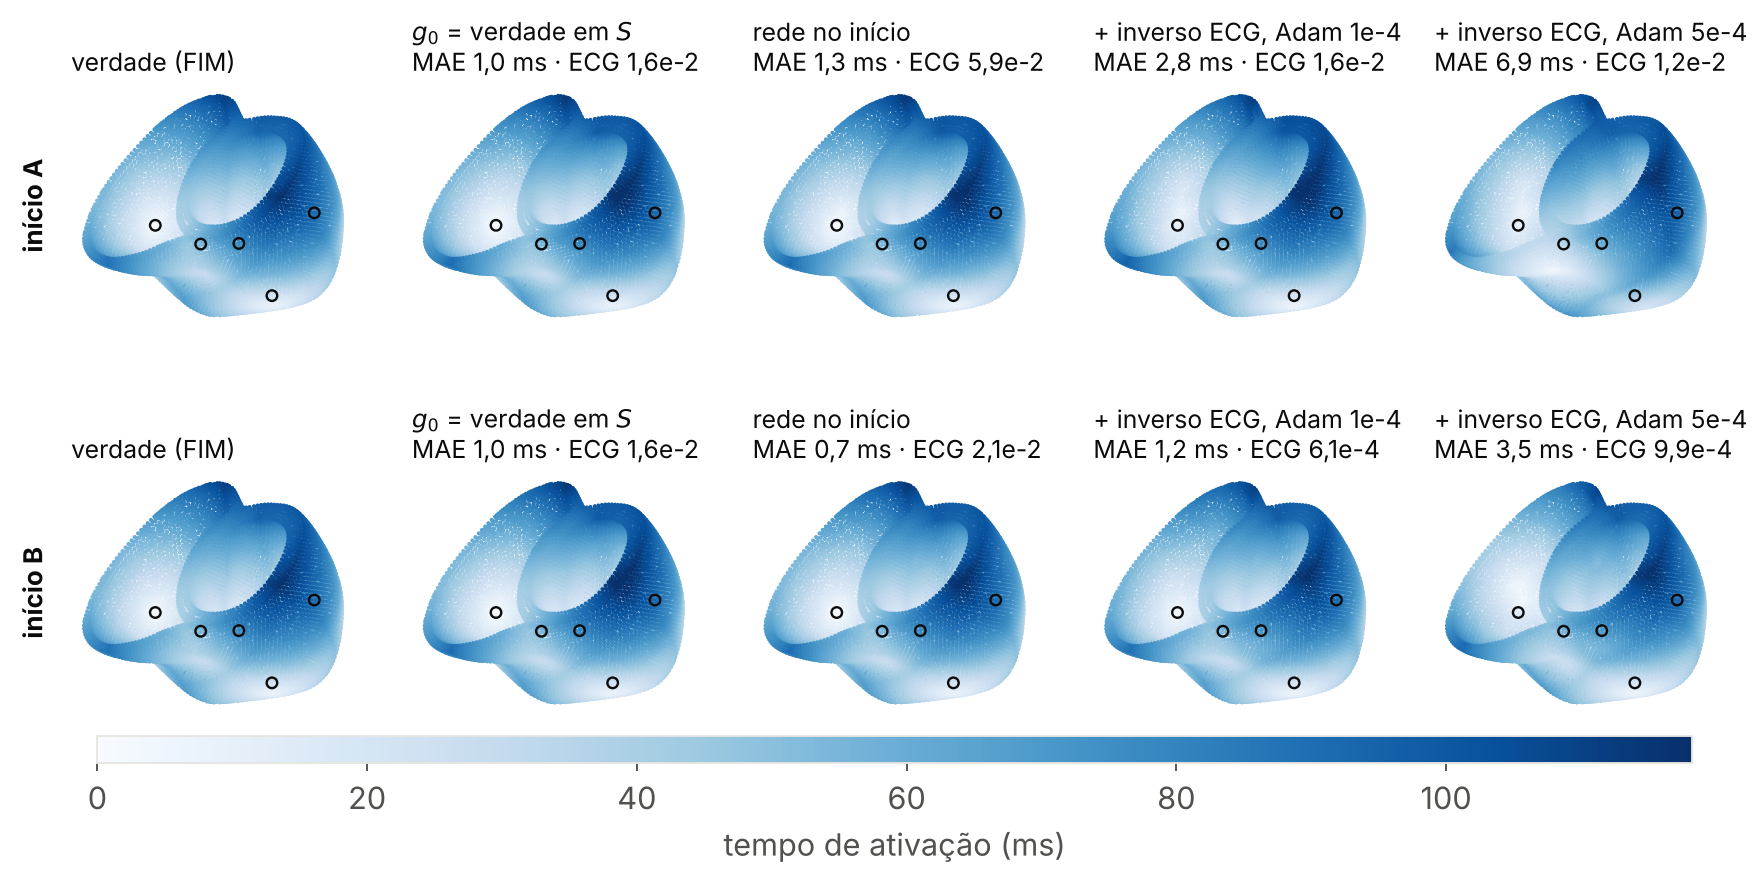
\includegraphics[width=0.97\linewidth]{hoje_mapas.png}
\end{frame}

\begin{frame}{Erro de LAT em cada estágio}
  \centering
  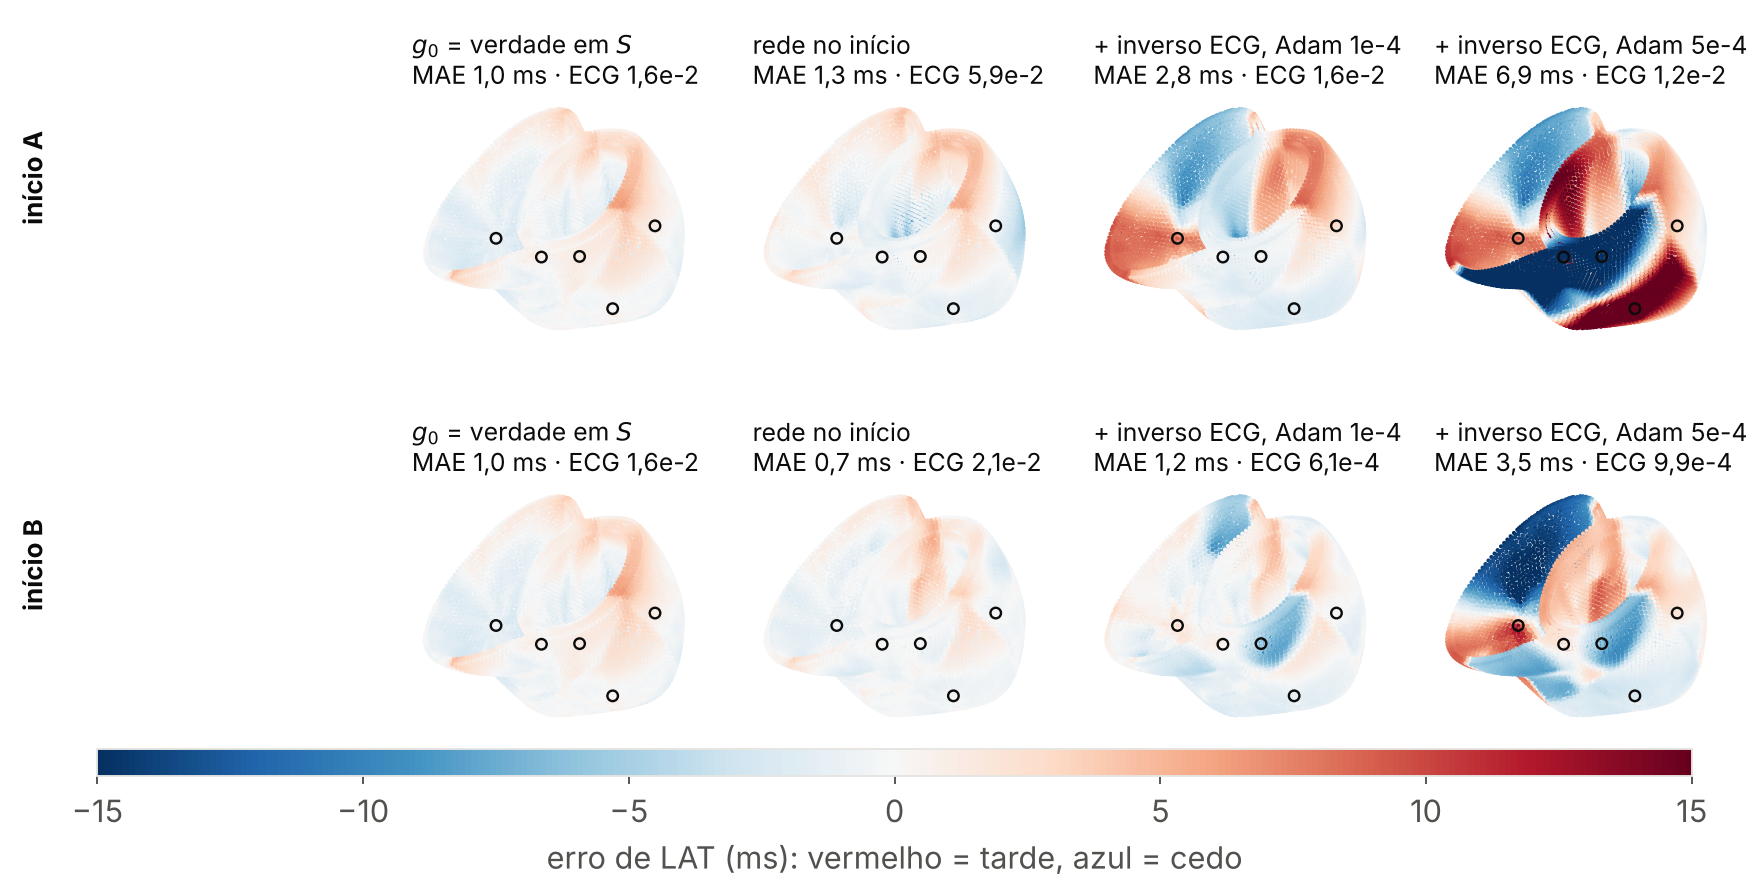
\includegraphics[width=0.97\linewidth]{hoje_erro.png}
\end{frame}

\begin{frame}{Sensibilidade ao ponto de partida}
  \centering
  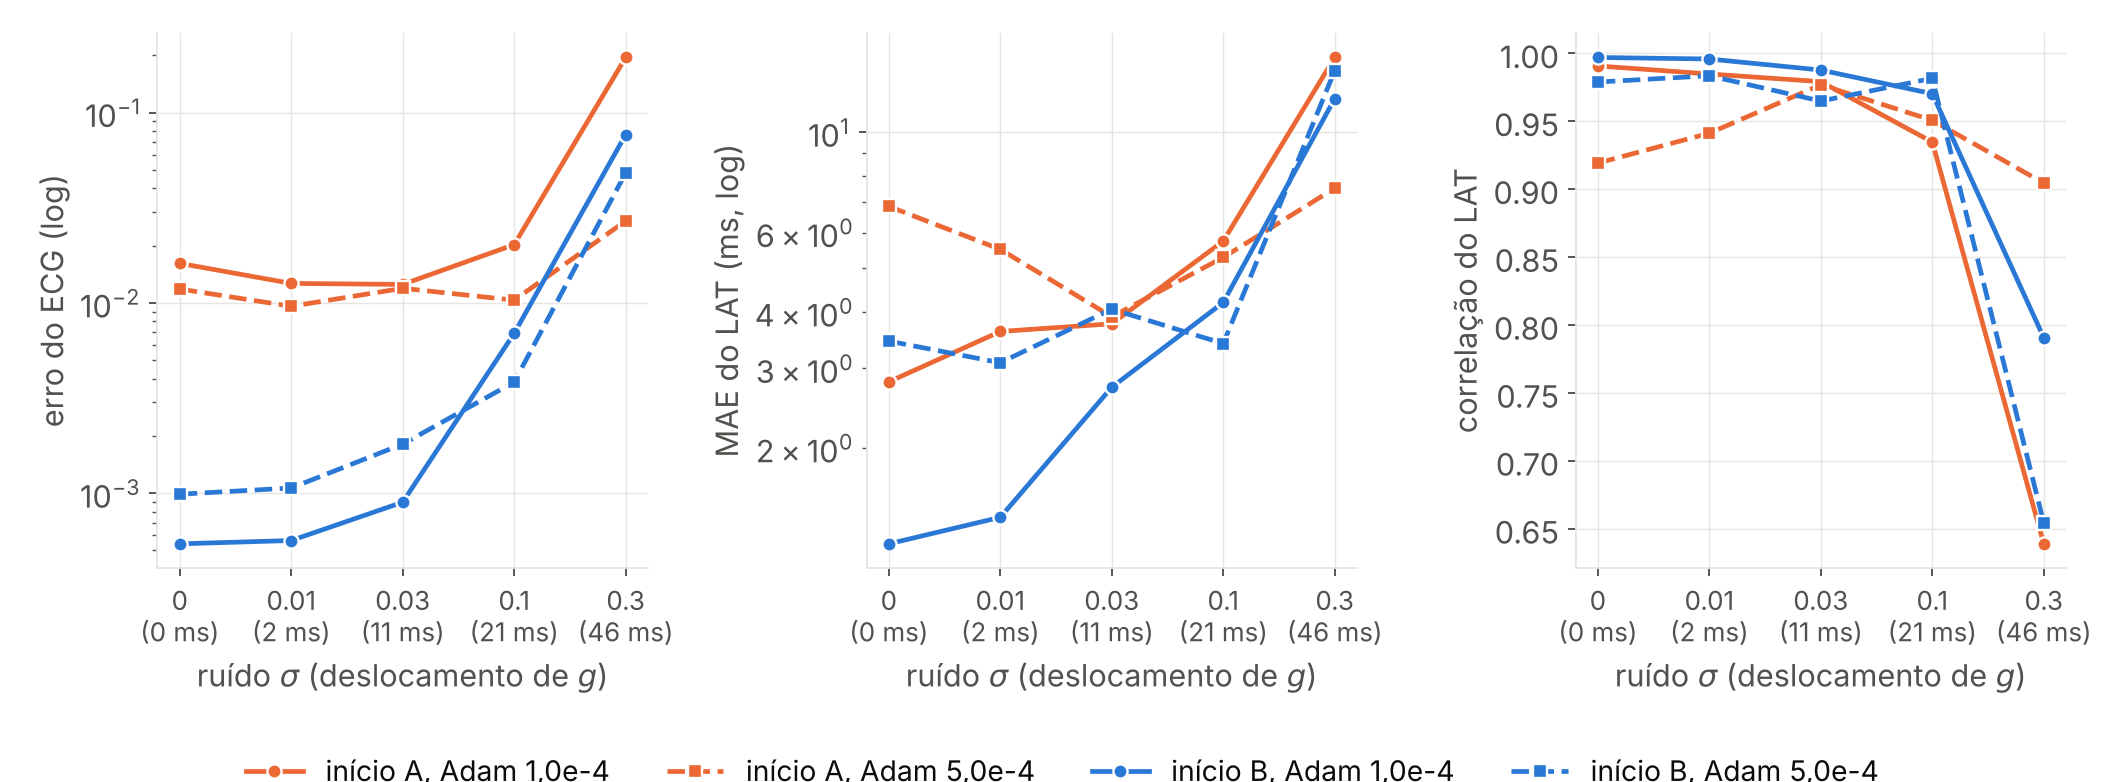
\includegraphics[width=\linewidth]{hoje_ruido.png}\par
  \smallskip
  {\scriptsize Ruído nos pesos da rede de início: $\sigma \times$ desvio de cada tensor; o mesmo ruído em A e B.
  Entre parênteses, quanto o ruído desloca $g$ nos candidatos dominantes. Mediana de 3 sorteios (1 em $\sigma = 0$).}
\end{frame}

\begin{frame}{Teste com $g$ conhecido: o alvo gerado pelo próprio Método 1}
  \centering
  \scriptsize
  \setlength{\tabcolsep}{4.5pt}
  \renewcommand{\arraystretch}{1.1}
  \begin{tabular}{@{}lcccccc@{}}
    \toprule
    início & \shortstack{ECG\\início} & \shortstack{ECG\\fim} & \shortstack{corr\\fim} & \shortstack{LAT MAE\\fim (ms)} & \shortstack{rms de $g$\\início (ms)} & \shortstack{rms de $g$\\fim (ms)}\\
    \midrule
\inputrows{sections/tab_gconhecido.tex}
    \bottomrule
  \end{tabular}\par
  \medskip
  {\tiny $g_{\mathrm{v}}$: o LAT verdadeiro em $S$; o mapa e o ECG alvo saem do Método 1 com $g_{\mathrm{v}}$ (erro zero é atingível).
  Ruído direto em $g$ (ms). Inverso só com ECG, Adam $5 \cdot 10^{-4}$, 1000 iterações.
  rms de $g$: nos 21 candidatos com $g_{\mathrm{v}} - \min < 10$ ms. Uma rodada por linha.}
\end{frame}
